\documentclass[]{IEEEtran}

\title{Modellazione e Sintesi di un Moltiplicatore Floating-point Single Precision}
\author{Enrico Sgarbanti - VR446095}

\usepackage{graphicx}
\usepackage{wrapfig}
\usepackage{hyperref}
\usepackage[italian]{babel}
\usepackage[utf8]{inputenc}

\begin{document}
\maketitle


\begin{abstract}
    Questo documento mostra la realizzazione di un moltiplicatore in virgola mobile a precisione singola realizzato in VHDL, Verilog e SystemC ed un componente che permetta di eseguire due moltiplicazioni in parallelo. Il tutto è accompagnato da testbench, sintesi dei componenti VHDL e verilog ed un confronto con l'High-level-Synthesis di un moltiplicatore scritto in c++.
\end{abstract}


\section{Introduzione}
Il sistema è composto da un modulo top-level chiamato ``double\_multiplier'' il quale esegue la moltiplicazione di due operandi dati in input nello stesso ciclo di clock in cui ready viene posto a 1, e i due opereandi passati al ciclo di clock successivo

Nell'introduzione viene descritto in maniera astratta quello che poi viene dettagliato nel seguito del report. Una buona scaletta per l'introduzione può essere la seguente:
\begin{itemize}
    \item Descrizione ad alto livello delle principali caratteristiche del sistema che si vuole modellare.
    \item Descrizione delle motivazioni principali per l'utilizzo delle tecnologie descritte nel corso. Qual è il problema che si vuole risolvere?
    \item Descrizione dei passi utilizzati per arrivare all'implementazione finale. Descrivere la motivazione di ciascun passo. La descrizione dei passi dovrebbe formare la descrizione del flusso di lavoro svolto per completare l'assignment.
    \item Rapidissima descrizione dei risultati principali.
\end{itemize}

L'introduzione non dovrebbe andare oltre la metà della seconda colonna (nel caso a due colonne), o la prima pagina (nel caso a colonna singola): bisogna cercare di essere concisi (e chiari). Alla fine, l'introduzione è solo ``chiacchiere'': deve semplicemente rendere chiari quali sono gli obiettivi del lavoro (\emph{e nel caso del corso, deve far capire a me che avete gli obiettivi chiari in testa}). Consiglio: l'introduzione (e spesso l'abstract) è l'ultima parte che viene completata.



\section{Background}

\subsection{Progettazione hardware}
Per la realizzazione di componenti hardware si possono utilizzare diverse tecniche e linguaggi.
Un primo approccio è descrivere i componenti a livello RT utilizzando linguaggi di descrizione hardware (HDL) come VHDL e Verilog.
Un HDL è un linguaggio specializzato per la descrizione della struttura e del comportamento di circuiti elettronici, in particolare circuiti logici digitali, e la loro analisi e simulazione. Permette inoltre la sintesi di una descrizione HDL in una netlist (una specifica di componenti elettronici fisici e il modo in cui sono collegati insieme), che può quindi essere posizionata e instradata per produrre l'insieme di maschere utilizzate per creare un circuito integrato\cite{HDL}.
\\Un secondo approccio è descrivere le funzionalità del componente con linguaggi più ad alto livello come C, C++ o SystemC\cite{SystemC} e fare High Level Syntesis (HLS) per ottenere una descrizione dell'hardware a livello RT\cite{HLS}.
\\Entrambi gli approcci hanno vantaggi e svantaggi. In particolare HLS riduce i tempi, ma la descrizione hardware generata sarà meno ottimizzata rispetto a quella che si potrebbe ottenere usando HDL.


\subsection{IEEE 754 single-precision binary floating-point format}
Questo standard definisce il formato per la rappresentazione dei numeri in virgola mobile (compreso $\pm 0$ e i numeri denormalizzati; gli infiniti e i NaN, "not a number"), ed un set di operazioni effettuabili su questi. 
\\In particolare la versione a precisione singola descrive il numero con 32 bit: 1 bit per segno (sign), 8 bit per l'esponente (esp) e 23 bit per la mantissa (mant)\cite{IEE754}.
\begin{figure}[!htb]
    \centering
    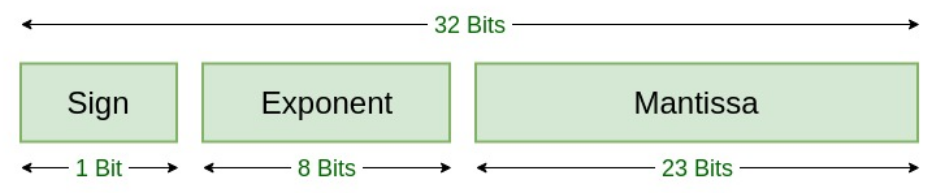
\includegraphics[width=0.9\linewidth]{figures/ieee754_single_precision.png}
    \caption{IEEE 754 single precision}
    \label{fig:IEE754}
\end{figure}
\\Per la codifica in numero binario:
\begin{itemize}
    \item Dal segno si ricava il bit più significativo (1 se negativato 0 altrimenti).
    \item Si converte il numero in binario.
    \item Si sposta la virgola a sinistra fino ad avere un numero nella forma $1,... \cdot 2^{E}$.
    \item La mantissa è la parte a destra della virgola, riempita con zeri a destra fino a riempire i 23 bit.
    \item L'esponente è $127+E$ dove E è l'esponente ricavato dallo shift.
\end{itemize}
Per la decodifica del numero binario: $$(-1)^{sign}\cdot 2^{(esp-127)} \cdot (1 + \sum_{i=1}^{23}b_{23-i}\cdot 2^{-i})$$
\begin{figure}[!htb]
    \centering
    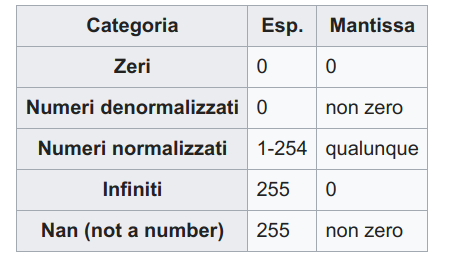
\includegraphics[width=0.6\linewidth]{figures/ieee754_special_case.png}
    \caption{IEEE 754 special case}
    \label{fig:IEEE_SPECIALCASE}
\end{figure}


\subsection{Moltiplicazione di due numeri floating-point}
Qui è riportato l'algoritmo usato per la moltiplicazione fra floating point. Guardare qui per ulteriori dettagli\cite{IEE754Mult}.
\begin{figure}[!htb]
    \centering
    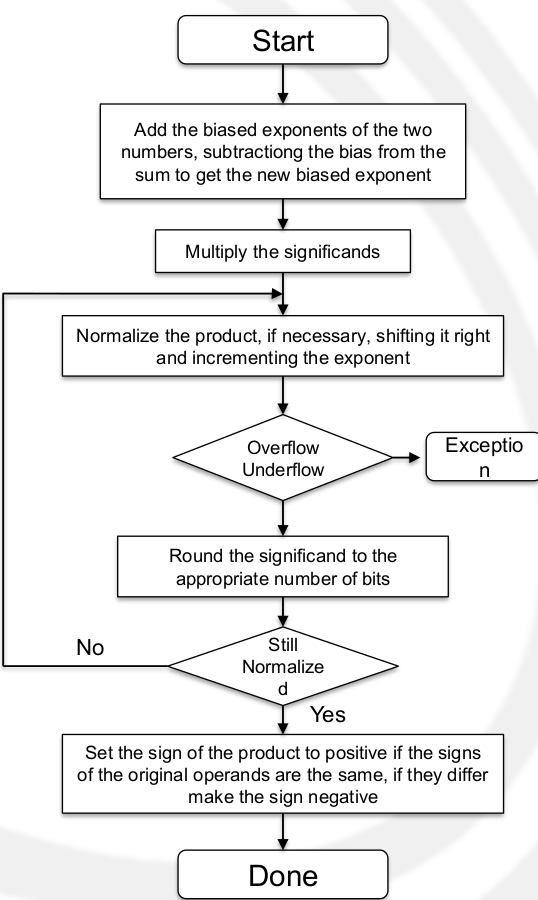
\includegraphics[width=0.6\linewidth]{figures/ieee_multiplication.png}
    \caption{IEEE 754 multiplication}
    \label{fig:IEEE_multiplication}
\end{figure}



\section{Metodologia applicata}
Il primo passo è stato la realizzazione della EFSM di \textit{multiplier} e \textit{double\_multiplier} che ha portato ad aquisire una visisione generale.
\\Dopo si è passati all'implementazione a livello RT con Vivado\cite{Vivado} del \textit{multiplier} sia in Verilog che in VHDL. Un primo test è stato fatto con TLC-script osservando gli output a determinati input.
\\Consolidati questi moduli è stato poi possibile realizzato in Verilog il \textit{double\_multiplier} che prende i due componenti e li usa per calcolare due moltiplicazioni. A questo punto è stato realizzato un test più accurato in verilog controllando tutti i casi particalari per poi passare alla sintesi.
\\È anche stato rifatto tutto in SystemC dove si è potuto fare un testbench più fine grazie alla potenza del c++.
\\Infine si è provato a fare l'high level syntesis da un semplice codice c++ per confrontare i risultati ottenuti.


\subsection{Vincoli ed Architettura}
Il progetto a diversi vincoli:
\begin{itemize}
    \item Il multiplier deve essere scritto in VHDL, verilog e systemC.
    \item Il double\_multiplier deve essere scritto in systemC e un linguaggio a scelta tra VHDL e verilog.
    \item Gli operandi e il risultato devono essere a 32 bit.
    \item I due componenti devono essere sintetizzabili sulla FPGA ``xc7z020clg400-1'' la quale ha a disposizione solo 125 porte.
\end{itemize}
Per far fronte al limite delle porte logiche è stato utilizzato il protocollo di handshake. Vengono quindi utilizzati gli stessi 32 bit per il risultato e altri 64 bit per le due coppie di operandi. Al primo ciclo di clock, con il flag ``ready'' uguale a 1, verranno trasmessi i primi due operandi e al ciclo successivo gli altri due. Dopodichè si aspetterà il complementanto delle moltiplicazioni, segnalato col flag ``done'' uguale a 1, per poi trasmettere il primo risultato, e il secondo al ciclo di clock successivo.
\\L'architettura con VHDL e Verilog è mostrata in figura \ref{fig:Architettura}. Quella per SystemC è analoga. 
\\I segnali intermedi sono stati omessi da questa figura, ma vengono descritti nelle sezioni successive.
\begin{figure}[!htb]
    \centering
    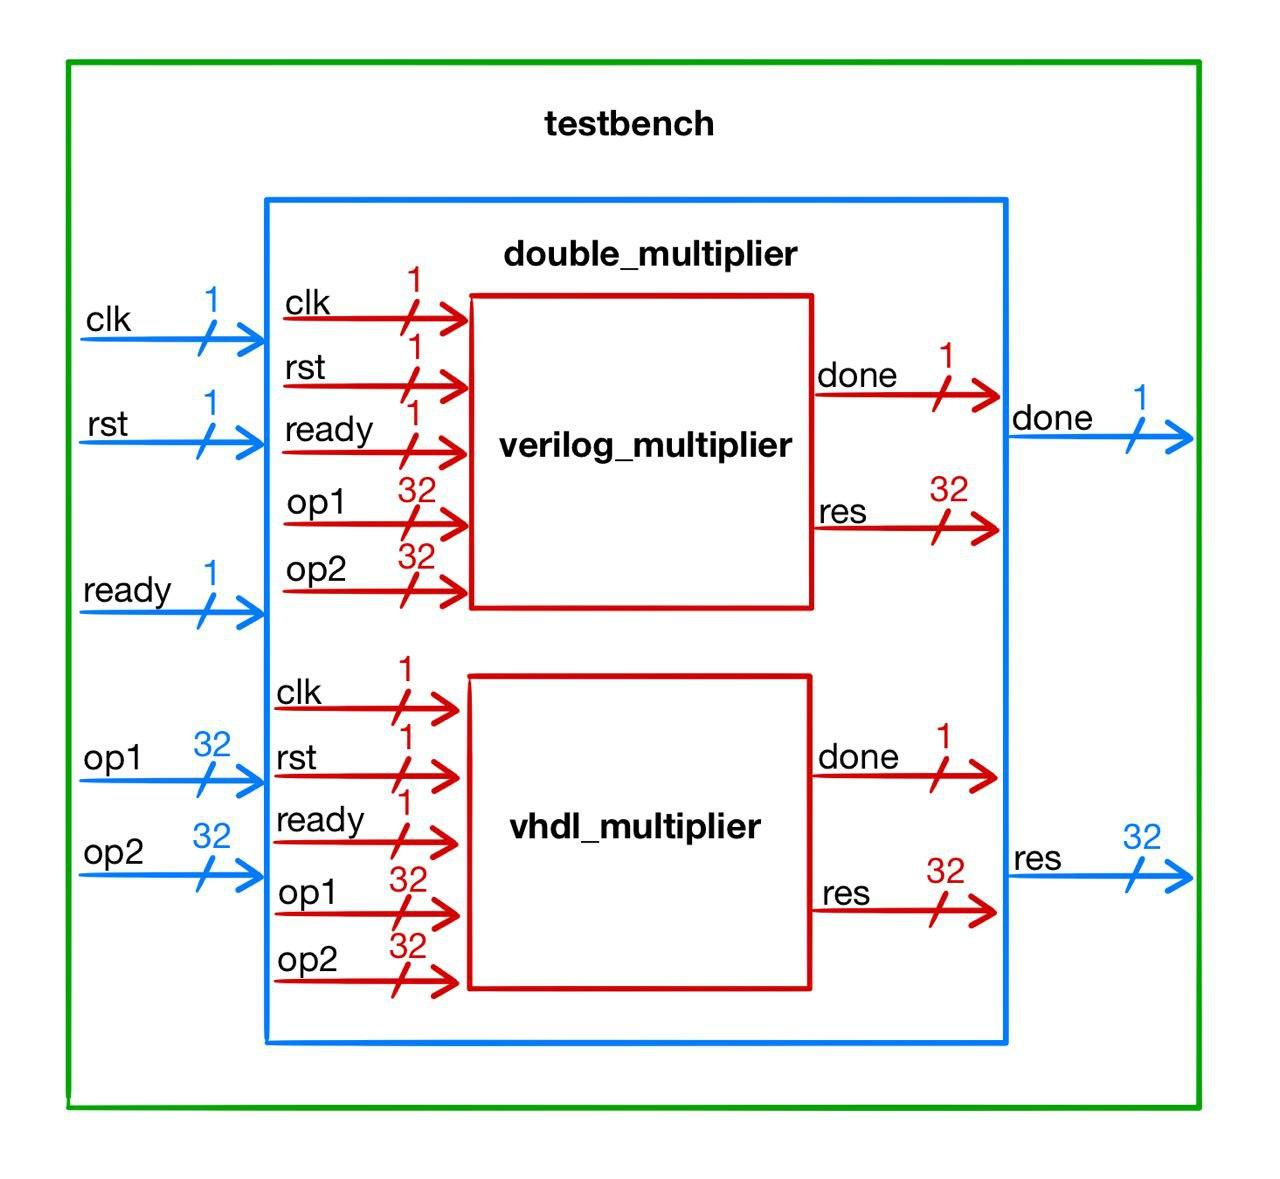
\includegraphics[width=0.6\linewidth]{figures/architettura.jpg}
    \caption{Architettura RTL}
    \label{fig:Architettura}
\end{figure}


\subsection{Modellazione della EFSM del multiplier [Figura \ref{fig:EFSM1}]}
Questo componente esegue la moltiplicazione tra numeri floating point a precisione singola.
\\I segnali intermedi utilizzati sono:
\begin{itemize}
    \item \textbf{rst} (1 bit): riporta il sistema allo stato iniziale.
    \item \textbf{ready} (1 bit): permette al sistema di uscire dallo stato iniziale.
    \item \textbf{norm\_again} (1 bit): indica che il numero ha bisogno di essere ulteriormente normalizzato.
    \item \textbf{res\_type} (2 bit): indicare il tipo del risultato. Solo nel caso in cui sia un numero si procede all'elaborazione, mentre negli altri casi si passa direttamente allo stato finale. Il caso del numero denormalizzato è gestito come se fosse normalizzato.
\end{itemize}

I registri intermedi utilizzati sono:
\begin{itemize}
    \item \textbf{STATE e NEXT\_STATE} (4 bit): rappresentano lo stato attuale e lo stato prossimo.
    \item \textbf{op1\_type e op2\_type} (2 bit): per indicare il tipo degli operandi ovvero 0, NaN, $\infty$ oppure un numero. Solo se sono entrambi sono dei numeri res\_type sarà un numero.
    \item \textbf{esp\_tmp} (10 bit): permette di eseguire le operazioni per ricavare l'esponente finale senza perdere informazioni.
    \item \textbf{mant\_tmp} (48 bit): permette di eseguire le operazioni per ricavare la mantissa finale senza perdere informazioni.
    \item \textbf{sign1, sign2, esp1, esp2, mant1, mant2}: rappresentano le componenti dei due operandi.
\end{itemize}

Sono  necessari 14 stati:
\begin{itemize}
    \item \textbf{ST\_START:} pone \textit{done} e \textit{norm\_again} a 0 ed estre le informazioni di segno, esponente e mantissa dei due operandi. Si rimane qui finchè \textit{ready} vale 0 altrimensi si passa a \textit{ST\_EVAL1}. Se in qualsiasi stato si riceve \textit{reset} uguale a 1 allora si passa a questo stato.
    \item \textbf{ST\_EVAL1 e ST\_EVAL2:} ricava rispettivamente il tipo di op1 e op2 fra \textit{T\_ZER, T\_INF, T\_NAN e T\_NUM}
    \item \textbf{ST\_EVAL3:} ricava il tipo del risultato in base al tipo di op1 e op2.
    \item \textbf{ST\_CHECK1:} controlla se \textit{res\_type} è uguale a T\_NUM e in tal caso passa a \textit{ST\_ELAB} altrimenti a \textit{ST\_FINISH}.
    \item \textbf{ST\_ELAB:} esegue la somma tra i due esponenti e la sottrazione di 127 in quanto entrambi, per lo standard, sono incrementati di 127: $(esp+127) = (esp1+127)+(esp2+127)-127$. Per compiere la somma è necessario usare una variabile \textit{esp\_tmp} di 10 bit perchè altrimenti con 8 bit si andrebbe in overflow con valori che dopo la sottrazione sarebbero rappresentabili con 8 bit e quindi validi. Viene poi eseguita anche la moltiplicazione delle due mantisse, che essendo a 23 bit più un bit che vale sempre 1, necessita di una variabile \textit{mant\_tmp} di almeno 48 bit
    \item \textbf{ST\_UNDERF:} controlla se \textit{esp\_tmp} è in uno stato di underflow, ovvero guardando se il bit \textit{esp\_tmp[9]}, che nel complemento a 2 indica il segno, è 1. Infatti i valori disponibili per l'esponente vanno da 0 a 255. Il controllo dell'overflow viene fatto in seguito all'arrotondamento per evitare di farlo due volte.
    \item \textbf{ST\_CHECK2:} passa allo stato \textit{ST\_FINISH} se \textit{res\_type} è diverso da \textit{T\_NUM}, perchè diventato \textit{T\_ZER} per l'underflow.
    \item \textbf{ST\_NORM1:} compie la normalizzazione della mantissa che deve sempre essere della forma \textit{1.bits}. Essendo la virgola posta tra il 46esimo bit e il 45esimo, si verificano due casi: Se il 47esimo bit vale 1 bisogna incrementare l'esponente, altrimenti il valore è già corretto, ma viene effettuato uno shift a sinistra per trattare allo stesso modo i due casi durante l'arrotondamento.
    \item \textbf{ST\_ROUND:} effettua l'eventuale arrotondamento dovuto al fatto che il valore della mantissa è attualmente a 48 bit, ma bisogna portarlo a 24 bit. L'arrotondamento è fatto per eccesso, quindi si incrementera \textit{mant\_tmp[47:24]} solo se \textit{mant\_tmp[23:00]} è $\geq$ a ``01..1''. L'arrotondamento effettivo verrà fatto nello stato \textit{ST\_NORM2}, qui ci si limita a porre \textit{norm\_again} uguale a 1 per poterci andare.
    \item \textit{\textbf{ST\_CHECK3:}} passa allo stato \textit{ST\_NORM2} se \textit{norm} è uguale a 1 oppure allo stato \textit{ST\_OVERF} se \textit{norm} è uguale a 0.
    \item \textbf{ST\_NORM2:} effettua il vero arrotondamento della mantissa. Bisogna tenere conto del caso in cui sia della forma ``1..1'' e che quindi con l'incremento vada a ``0..0'' e  venga incrementato l'esponente.
    \item \textbf{ST\_OVERF:} verifica se l'esponente del risultato è in uno stato di overflow, ovvero guardando se il bit \textit{esp\_tmp[8]} vale 1 ovvero se corrisponde ad un valore maggiore di 255.
    \item \textbf{ST\_FINISH:} pone \textit{done} uguale 1 e ricava \textit{res[31]}, ovvero il segno del risultato facendo lo XOR fra i segni degli operandi. In base al valore di \textit{res\_type} si ricavano gli altri bits e si torna allo stato iniziale.
\end{itemize}


\subsection{Modellazione della EFSM del double\_multiplier (textit{Figure \ref{fig:EFSM2}})}
I segnali utilizzati per la comunicazione sono:
\begin{itemize}
    \item \textbf{rst:} (1 bit) per riportare il sistema allo stato iniziale .
    \item \textbf{ready:} (1 bit) per permettere al sistema di uscire dallo stato iniziale .
    \item \textbf{done1:} (1 bit) che indica quando il valore attuale di ``res1'' è il risultato della moltiplicazione.
    \item \textbf{done2:} (1 bit) che indica quando il valore attuale di ``res2'' è il risultato della moltiplicazione.
\end{itemize}

Sono inoltre necessari 8 stati:

\begin{itemize}
    \item \textbf{ST\_START:} in cui si pone textit{done}, textit{ready1} e textit{ready2}uguali a 0 e si inizializzano textit{op1\_tmp1} e textit{op2\_tmp1} rispettivamenete con i valori di textit{op1} e textit{op2} i quali serviranno per il primo moltiplicatore. In esso si rimane finchè textit{ready} vale 0 altrimensi si passa a textit{ST\_RUN1}.
    \item \textbf{ST\_RUN1:} in cui si pone textit{ready1} uguale a 1, attivando quindi il primo moltiplicatore, e si inizializzano textit{op1\_tmp2} e textit{op2\_tmp2} rispettivamenete con i valori di textit{op1} e textit{op2} i quali serviranno per il secondo moltiplicatore.
    \item \textbf{ST\_RUN2:} in cui si pone textit{ready1} uguale a 0 e textit{ready2} uguale a 1, attivando quindi il secondo moltiplicatore
    \item \textbf{ST\_WAIT:} in cui si pone textit{ready2} uguale a 0 e si aspetta che textit{done1} o textit{done2} diventino 1.
    \item \textbf{ST\_WAIT1:} si arriva in questo stato se textit{done2} vale 1, cioè se il secondo moltiplicatore ha finito e si resta qui finchè non finisce anche il primo.
    \item \textbf{ST\_WAIT2:} si arriva in questo stato se textit{done1} vale 1, cioè se il primo moltiplicatore ha finito e si resta qui finchè non finisce anche il secondo.
    \item \textbf{ST\_RET1:} si arriva in questo stato quando entrambi i moltiplicatore hanno finito. Qui si pone textit{done} uguale a 1 e textit{res} uguale al risultato del primo moltiplicatore cioè textit{res1}.
    \item \textbf{ST\_RET2:} ora si pone textit{res} uguale al risultato del secondo moltiplicatore cioè textit{res2} e si ritorna allo stato iniziale.
\end{itemize}


\subsection{Implementazione RTL}
L'intefaccia del textit{double\_multiplier} è formata dai segnali di input: textit{clk, rst, ready, op1, op2}; E i segnali di output textit{res, done}. \\
L'intefaccia del textit{multiplier} è formata anch'essa dai segnali di input: textit{clk, rst, ready, op1, op2}; E i segnali di output textit{res, done}, dove:
\begin{itemize}
    \item textit{clk, rst} sono collegati ai segnali analoghi del textit{double\_multiplier}.
    \item textit{ready} è collegato al segnale interno del textit{double\_multiplier} textit{ready1}, per multiplier1 e textit{ready2} per multiplier2.
    \item textit{op1 e op2} sono collegati ai segnali interni del textit{double\_multiplier} textit{op1\_tmp1, op2\_tmp1}, per multiplier1 e textit{op1\_tmp1, op2\_tmp2} per multiplier2.
    \item textit{res} è collegato al segnale interno del textit{double\_multiplier} textit{res1}, per multiplier1 e textit{res2} per multiplier2.
    \item textit{done} è collegato al segnale interno del textit{double\_multiplier} textit{done1}, per multiplier1 e textit{done2} per multiplier2.
\end{itemize}
textit{op1\_tmp1, op2\_tmp1, op1\_tmp2, op2\_tmp2} sono necessari al fine di conservare i valori della prima coppia di operandi e della seconda, che verranno passati ai moltiplicatori dei cicli di clock dopo. \\
La FSMD è realizzata con due processi:
\begin{itemize}
    \item fsm: processo asincrono attivato con la variazione di qualche segnale interno. Esso ha il compito di calcolare e aggiornare lo stato prossimo ``NEXT\_STATE''.
    \item datapath: processo sincrono che ha il compito di aggiornare lo stato attuale, elaborare gli output. Esso viene anche attivato dal fronte di salita del reset al fine di riportare lo stato a quello iniziale.
\end{itemize}


\subsection{Implementazione RTL con Verilog e VHDL}
Si creano i seguenti files:
\begin{itemize}
    \item \textbf{verilog\_multiplier:} implementazione verilog del moltiplicatore (sintetizzabile)
    \item \textbf{vhdl\_multiplier:} implementazione vhdl del moltiplicatore (sintetizzabile)
    \item \textbf{double\_multiplier:} implementazione verilog del doppio moltiplicatore (sintetizzabile)
    \item \textbf{testbench:} implementazione verilog di un testbench da usare solo in simulazione
\end{itemize}
In textit{verilog\_multiplier} e textit{double\_multiplier}
\begin{itemize}
    \item Sono definiti come ``wire'' tutti i segnali collegati alle porte di input mentre come ``reg'' tutti quelli collegati alle porte di output.
    \item Sono definiti come ``reg'' tutti i segnali interni di communicazione.
    \item Gli stati e textit{op1\_type, op2\_type, res\_type} sono stati definiti come ``parameter''.
\end{itemize}
In textit{vhdl\_multiplier:}
\begin{itemize}
    \item Sono usate le librerie ``IEEE.STD\_LOGIC\_1164.ALL'' per abilitare i tipi std\_logic e ``use IEEE.NUMERIC\_STD.ALL'' per usare funzioni aritmetiche con valori signed e unsigned
    \item Sono definiti come ``signal'' tutti i segnali collegati alle porte di input e output.
    \item Sono definiti come ``signal'' tutti i segnali interni di communicazione.
    \item Sono definite come ``variable'' textit{sign1, sign2, esp1, esp2, esp\_tmp, mant1, mant2, mant\_tmp, op1\_type, op2\_type} perchè utilizzati solo all'interno del processo ``datapath''.
    \item Gli stati e textit{op1\_type, op2\_type, res\_type} sono stati definiti all'interno del textit{package} rispettivamente come ``MULT\_STATE'' e ``MULT\_TYPE''.
    \item L'architettura utilizzata segue lo stile ``behavioral'', cioè quello più ``program-like'' in quanto più semplice e chiaro per descrivere una FSMD con due processi.
\end{itemize}



\subsection{Implementazione RTL con SystemC}
Si creano i seguenti files e directory:
\begin{itemize}
    \item \textbf{Makefile:} tool per la compilazione automatica del progetto. Richiede che la variabile d'ambiente SYSTEMC\_HOME contenga il path alla libreria di SystemC.
    \item \textbf{bin:} directory che contiene l'eseguibile textit{double\_multiplier\_RLT.x} (generato dopo la compilazione) e textit{wave.vcd} (generato dopo l'esecuzione dell'eseguibile).
    \item \textbf{obj:} directory che contiene i files oggetto (generati dopo la compilazione)
    \item \textbf{include:} directory che contiene gli headers textit{double\_multiplier\_RTL.hh}, textit{multiplier\_RTL.hh}, textit{testbench\_RTL.hh}. Qui sono definite tutte le porte, segnali, variabili ed enumerazioni dei vari componenti
    \item \textbf{testbench:} directory che contiene i files sorgenti textit{double\_multiplier\_RTL.cc}, textit{multiplier\_RTL.cc}, textit{testbench\_RTL.cc} e textit{main\_RTL.cc}.
\end{itemize}
In textit{double\_multiplier\_RTL.hh}
\begin{itemize}
    \item Sono definiti come ``sc\_signal'' tutti i segnali collegati alle porte di input e output.
    \item Sono definiti come ``sc\_signal'' tutti i segnali interni di communicazione.
    \item Gli stati sono stati definiti come ``enumerazioni''.
\end{itemize}
In textit{multiplier\_RTL.hh}
\begin{itemize}
    \item Sono definiti come ``sc\_signal'' tutti i segnali collegati alle porte di input e output.
    \item Sono definiti come ``sc\_signal'' tutti i segnali interni di communicazione.
    \item Sono definite come variabili di SystemC textit{sign1, sign2, esp1, esp2, esp\_tmp, mant1, mant2, mant\_tmp, op1\_type, op2\_type} perchè utilizzati solo all'interno del processo ``datapath''.
    \item Gli stati e textit{op1\_type, op2\_type, res\_type} sono stati definiti come ``enumerazioni''.
\end{itemize}
A differenza di verilog e VHDL, in SystemC è necessario un file ``main'' che contenga il metodo textit{sc\_main} e che permetta di collegare il componente da testare con il testbench. In esso si utilizza textit{sc\_create\_vcd\_trace\_file} per salvare le tracce necessarie a lanciare una simulazione con tools come gtkwave.


\section{Risultati}
Il testbench verilog, textit{Figure \ref{fig:SIM1}}, aspetta un po di tempo, perchè altrimenti si verificherebbero problemi dovuti allo startup della FPGA nella simulazione post-sintesi, e poi esegue due volte il textit{double\_multiplier}, prima con due coppie di operandi che danno come risultato dei numeri normali, e poi con due coppie di operandi che danno come risultati dei casi speciali. \\

Il testbench in SystemC mette a disposizione tre thread da attivare togliendo i commenti nel costruttore del ``TestbenchModule'':
\begin{itemize}
    \item \textbf{targeted\_test:} che analogamente a quello in Verilog, testa due volte il textit{double\_multiplier}. textit{Figure \ref{fig:SIM2}}.
    \item \textbf{rnd\_test:} che prova textit{TESTS\_NUM} moltiplicazioni generate casualmente tra un intervallo modificabile. textit{Figure \ref{fig:SIM3}}.
    \item \textbf{run\_all:} che prova tutte le possibili combinazioni cioè \(2^{32} * 2^{32}\). Si può limitare il numero di combinazioni evitando di contare il bit del segno, in quanto il calcolo è un semplice xor. Poi si possono escludere tutti i numeri denormalizzati. Ma anche così il tempo necessario a completarlo è troppo elevato per la mia macchina.
\end{itemize}
Con la sintesi si sono ottenuti i seguenti risultati:


















Questa sezione può contenere anche riflessioni personali sui risultati ottenuti. Importante: tutte le affermazioni devono essere supportate da numeri\footnote{Richard Feynman on Scientific Method (1964) -\\ https://www.youtube.com/watch?v=OL6-x0modwY}.

\section{Conclusioni}
Le conclusioni dovrebbero riassumere in poche righe  tutto ciò che è stato fatto. Un paio di righe descrivono i risultati osservati, in modo da introdurre poi la conclusione ``vera e propria''. Nel caso del corso, la ``lezione da portare a casa'' sarà quello che si è imparato svolgendo l'elaborato.


\bibliographystyle{IEEEtran}
\bibliography{biblio}
\appendix

\begin{figure*}[bt]
    \centering
    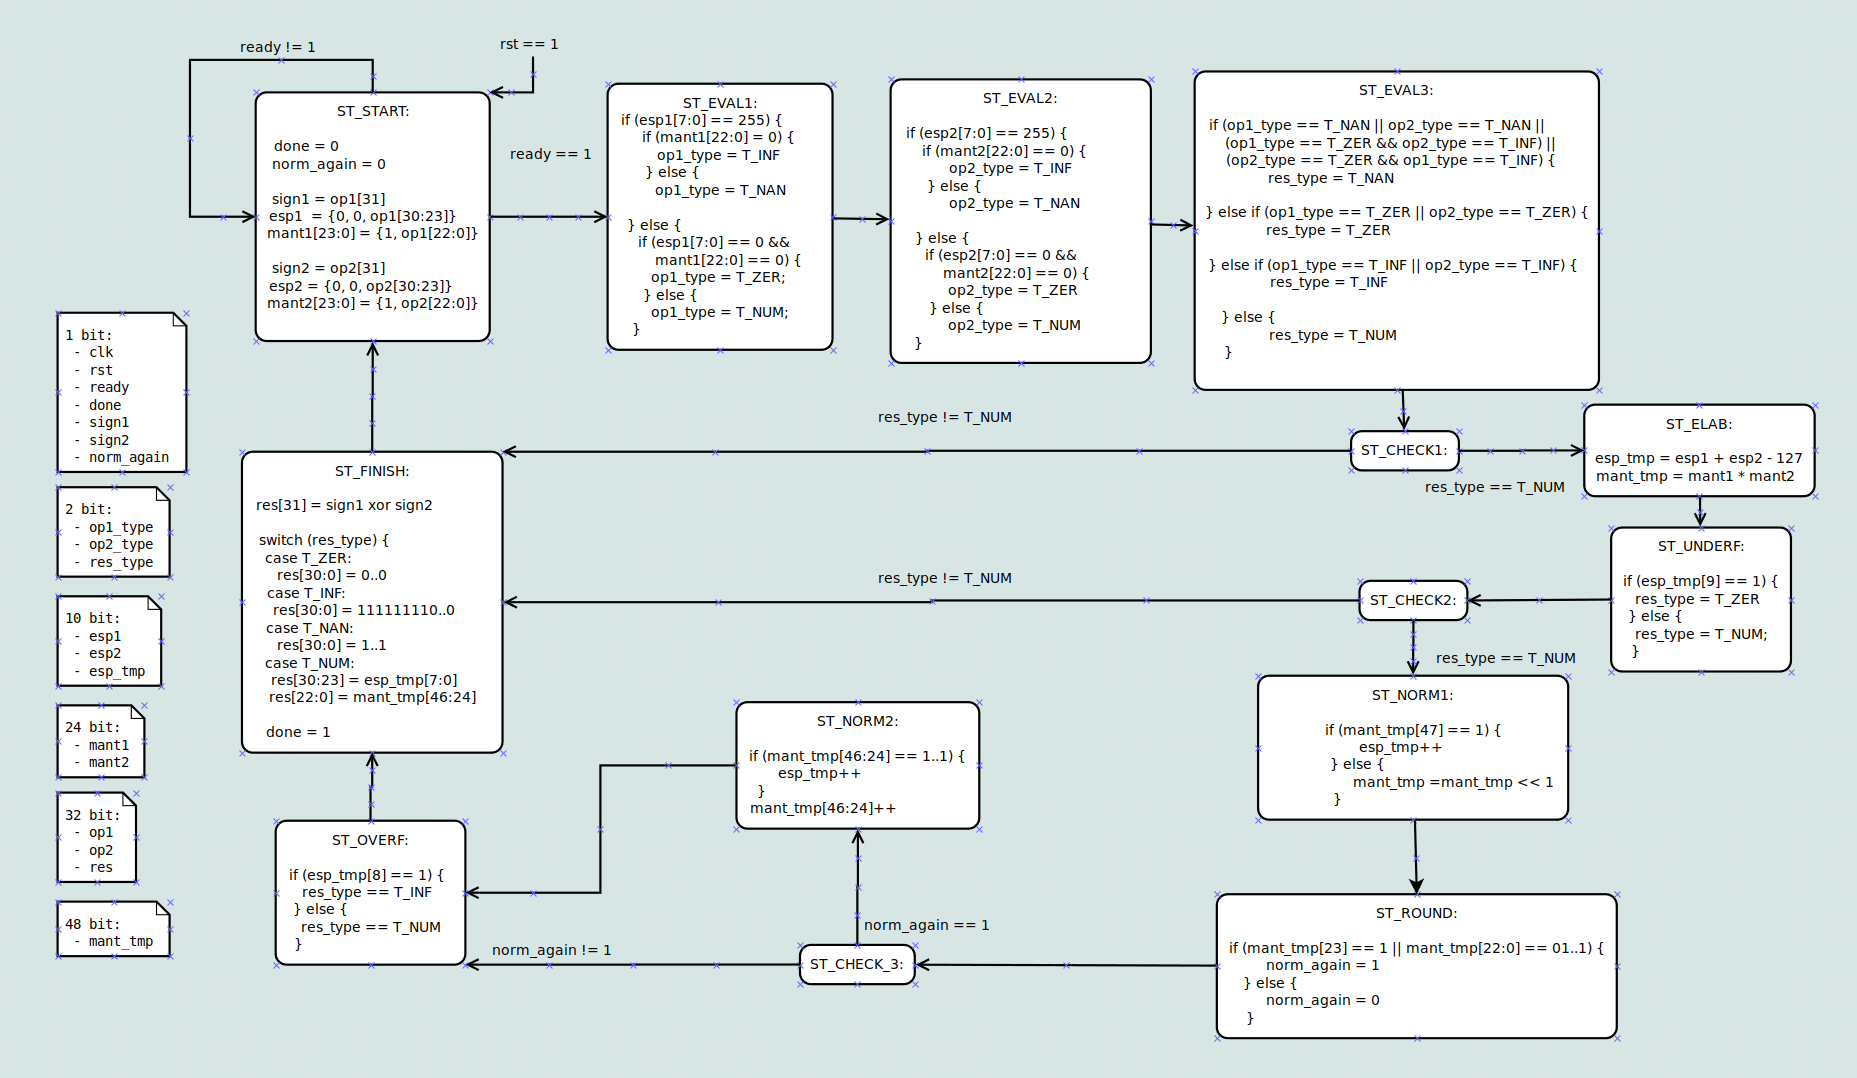
\includegraphics[width=\textwidth]{figures/EFSM-multiplier}
    \caption{EFSM del multiplier}
    \label{fig:EFSM1}
\end{figure*}

\begin{figure*}[bt]
    \centering
    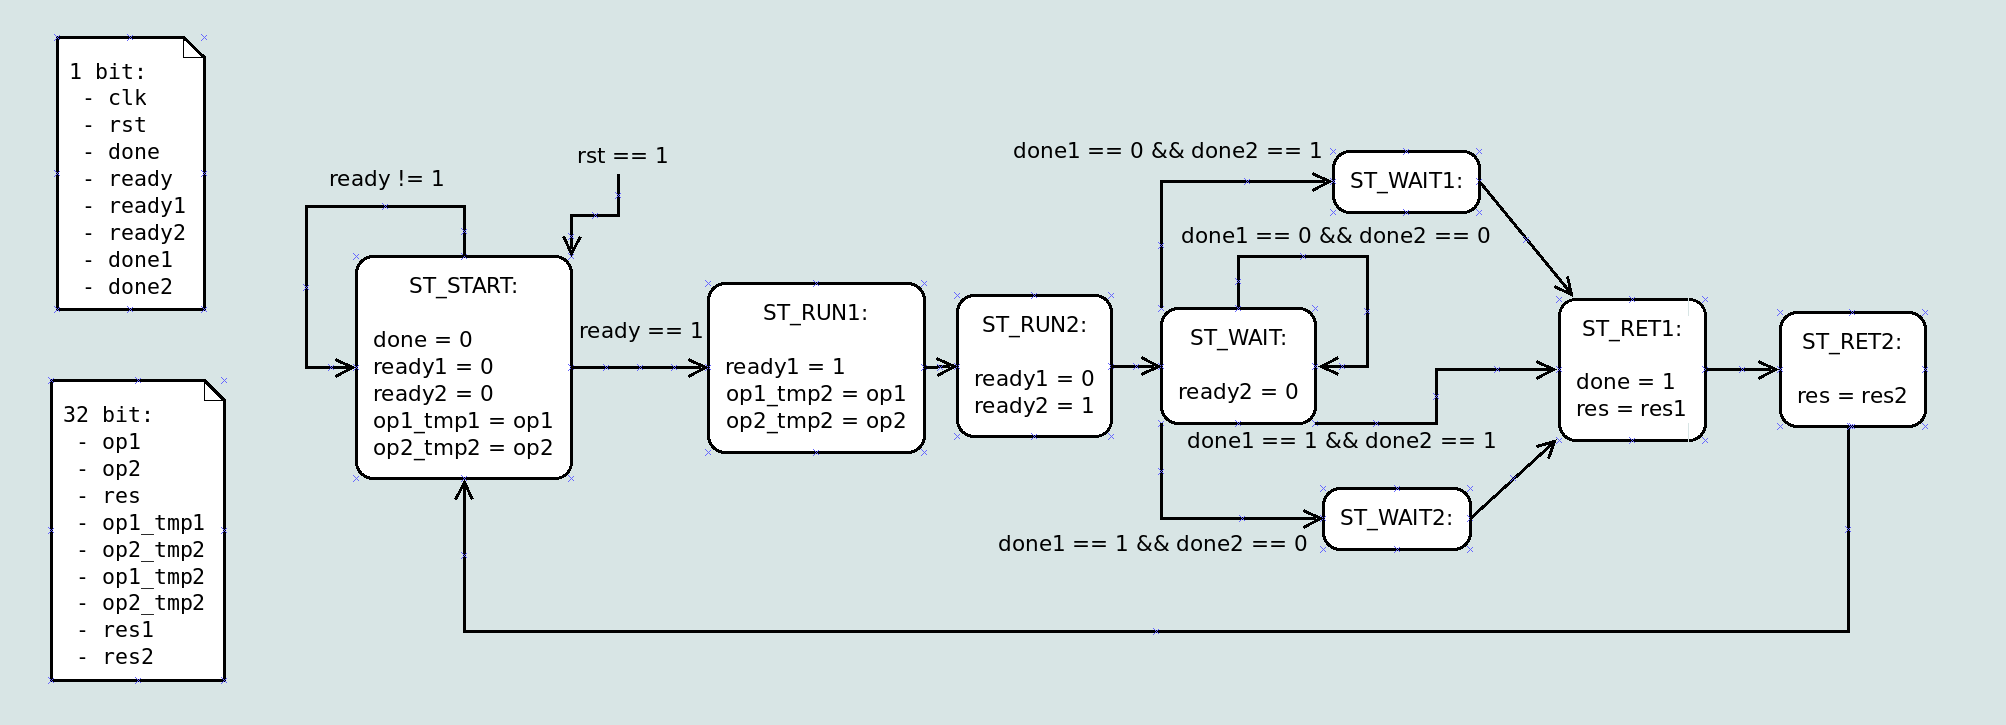
\includegraphics[width=\textwidth]{figures/EFSM-top_level}
    \caption{EFSM del double\_multiplier}
    \label{fig:EFSM2}
\end{figure*}

\begin{figure*}[bt]
    \centering
    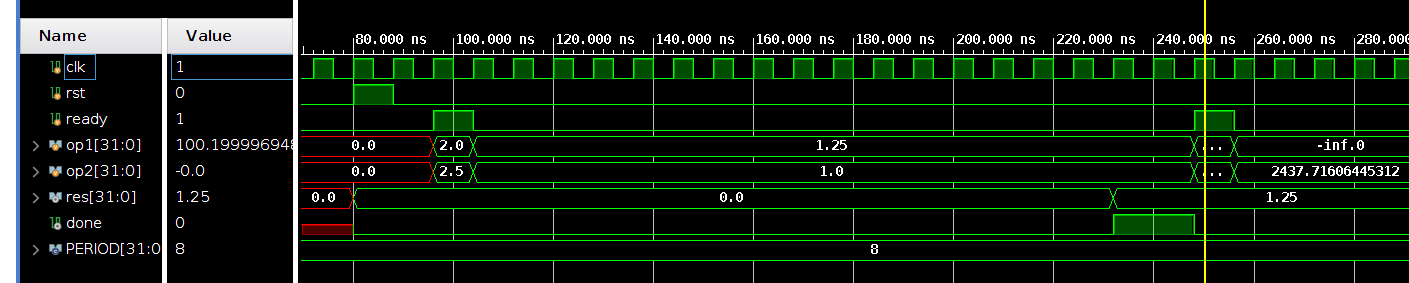
\includegraphics[width=\textwidth]{figures/simulazione1}
    \caption{Simulazione in Verilog}
    \label{fig:SIM1}
\end{figure*}

\begin{figure*}[bt]
    \centering
    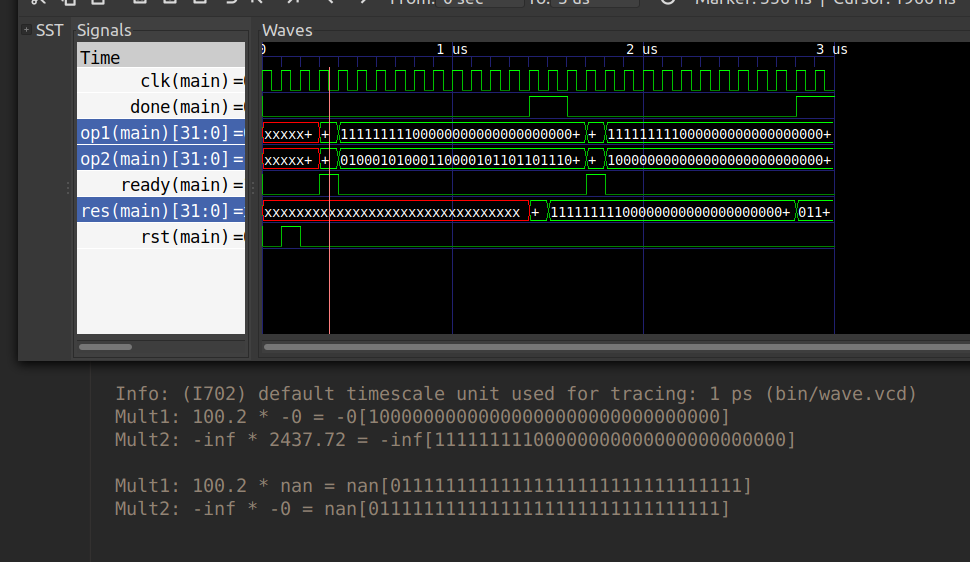
\includegraphics[width=\textwidth]{figures/simulazione2}
    \caption{Simulazione in SystemC con targeted\_test}
    \label{fig:SIM2}
\end{figure*}

\begin{figure*}[bt]
    \centering
    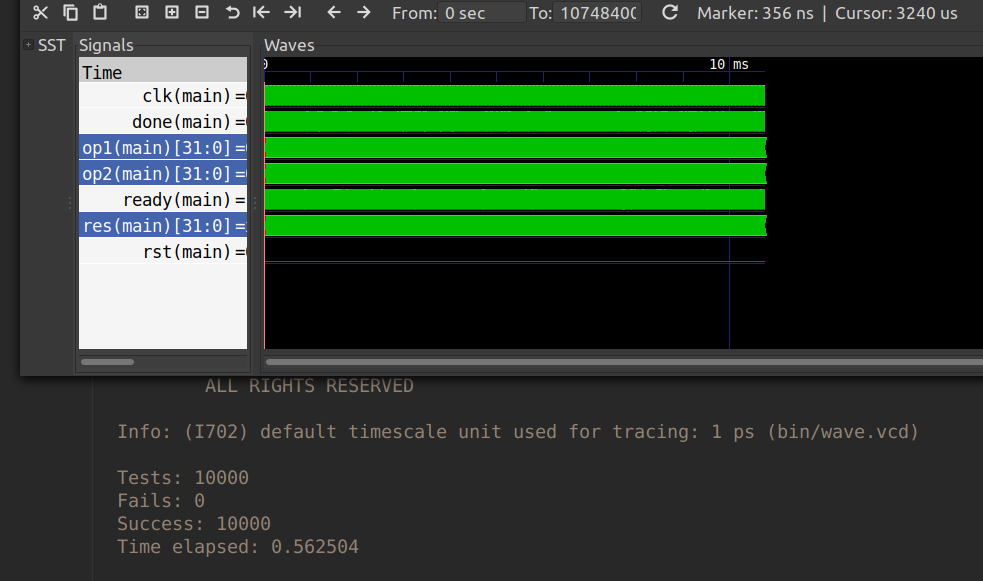
\includegraphics[width=\textwidth]{figures/simulazione3}
    \caption{Simulazione in SystemC con rnd\_test}
    \label{fig:SIM3}
\end{figure*}

\end{document}